\documentclass[12pt,a4paper]{article}
\usepackage[utf8]{inputenc}
\usepackage[T1]{fontenc}
\usepackage{amsmath}
\usepackage{amsfonts}
\usepackage{amssymb}
\usepackage{amsthm}
\usepackage{graphicx}
\usepackage{subfigure}
\usepackage{float}
\newtheorem*{theorem}{Theorem}
\newtheorem*{prf}{\textbf{Proof}}
\usepackage{caption}
\DeclareMathOperator{\xyz}{\textbf{numpy.random.normal()}}
\title{CS331-HW3-Lukang-Sun}
\begin{document}
	\maketitle
	\paragraph{p1.}
	Let's write the Lagrangian for this optimization problem: $L(p_1,\cdots,p_n,\lambda) = \sum_{i=1}^{n} \frac{a_{i}}{p_{i}}+\lambda (\sum_{i=1}^{n}p_i-1.)$ Next, we should equate to zero the derivative with respect to each $p_i,\text{for } i=1,\cdots, n$,
	\begin{equation}
			\nabla_{p_i}L(p_1,\cdots,p_n,\lambda) = -\frac{a_i}{p_i^2}+\lambda = 0 \Rightarrow p_i = \sqrt{\frac{a_i}{\lambda}},
	\end{equation}
   we also need $\sum_{i=1} ^{n}p_i=1$, combine this with (1), we reach $\sqrt{\lambda} = \sum_{i=1}^{n}\sqrt{a_i}$, finally use (1) again, we have $p_{i}=\frac{\sqrt{a_{i}}}{\sum_{j} \sqrt{a_{j}}}.$


\paragraph{p2.}
In my experiments(see Figure \ref{img1}.), I set $g(x,y) = 0.02x^2+y^2$, $L = \left[2,4,6,3,2,9,6,7,11,45\right], f_i(x,y) = 0.5L_ig(x,y), f(x,y) = 0.1\sum_{i=0}^{9}f_i(x,y)$, step size for SGD-US is $\frac{1}{\max_iL_i} = \frac{1}{45}$, for SGD-IS is $\frac{1}{10\sum_{i=0}^{9}L_i}=\frac{1}{9.5}$. We can  see that $\frac{\max_iL_i}{\sum_{i=0}^{9}L_i}\approx 4.74$, so SGD-IS should approximately converge to the minimum point with much fewer steps than SGD-US should do, actually, this is demonstrated by my simulations. Due to my design of optimization function, you can not observe randomness in the trajectories of SGD-IS, while in the trajectories of SGD-US there is randomness. I run 100 times to estimate the mean error that is $\text{Error} = E\left[||x_{iteration}||^2\right]\approx \frac{1}{100}\sum_{i=1}^{100} ||x_{iteration}^i||^2$, $x_{iteration}^i$ is the i-th sample of the last iteration point.

\begin{figure}
	\centering
	\subfigure[ ]{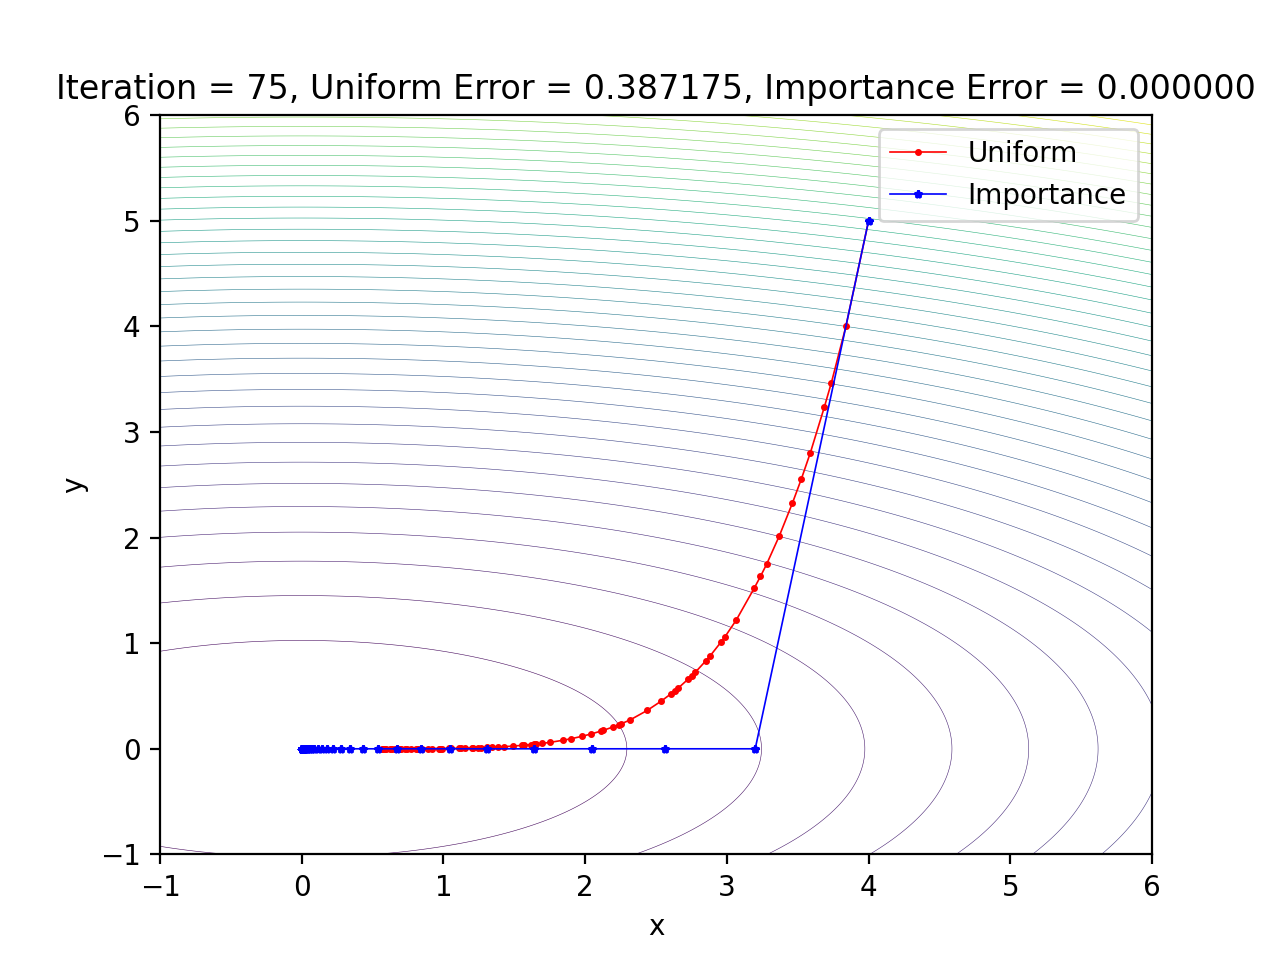
\includegraphics[width=6.7cm]{Figure_32.png}} 
	\subfigure[]{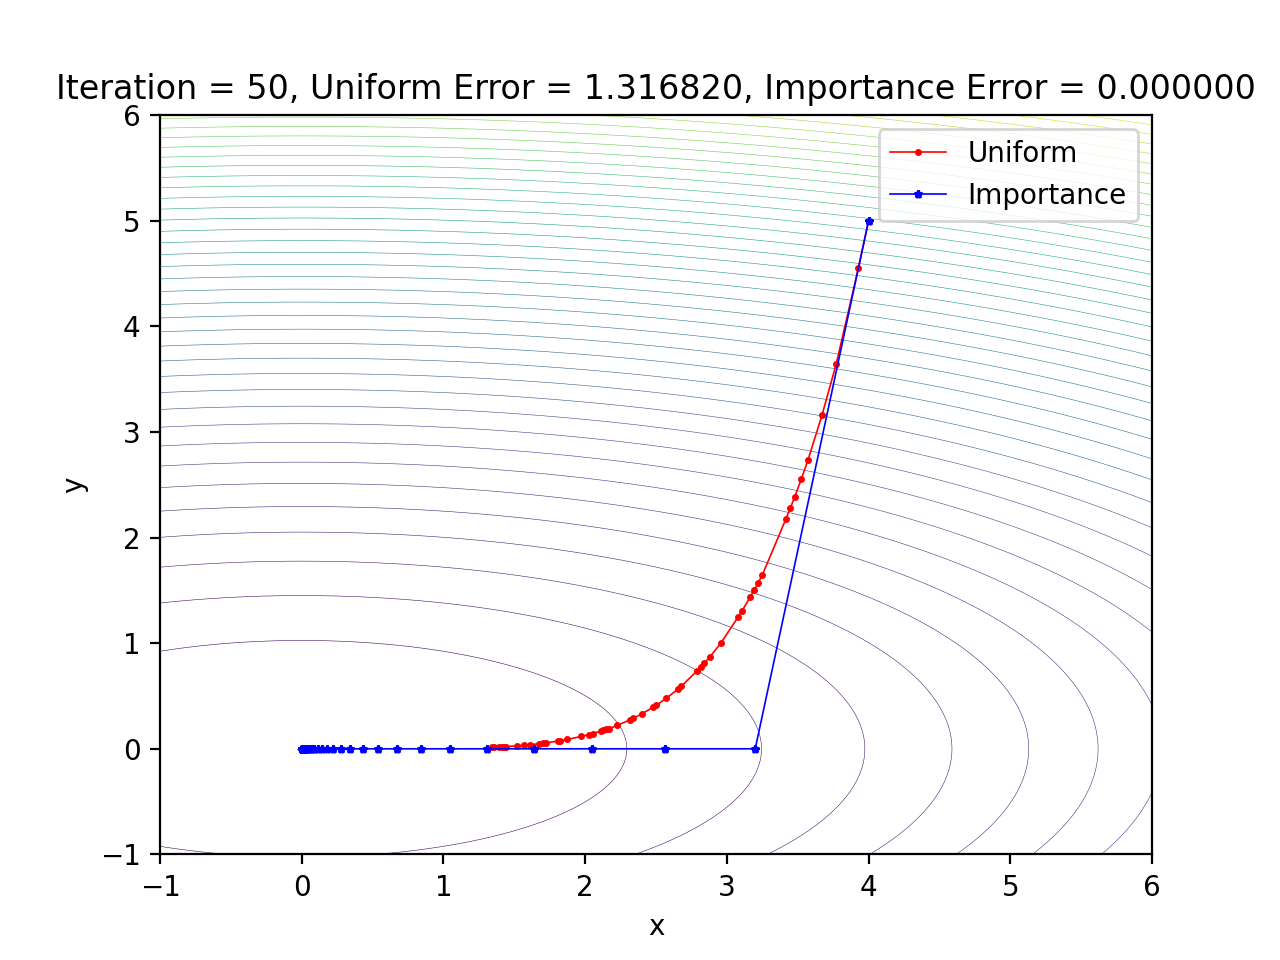
\includegraphics[width=6.7cm]{Figure_33.png}}
	\\ %换行
	\centering
	\subfigure[]{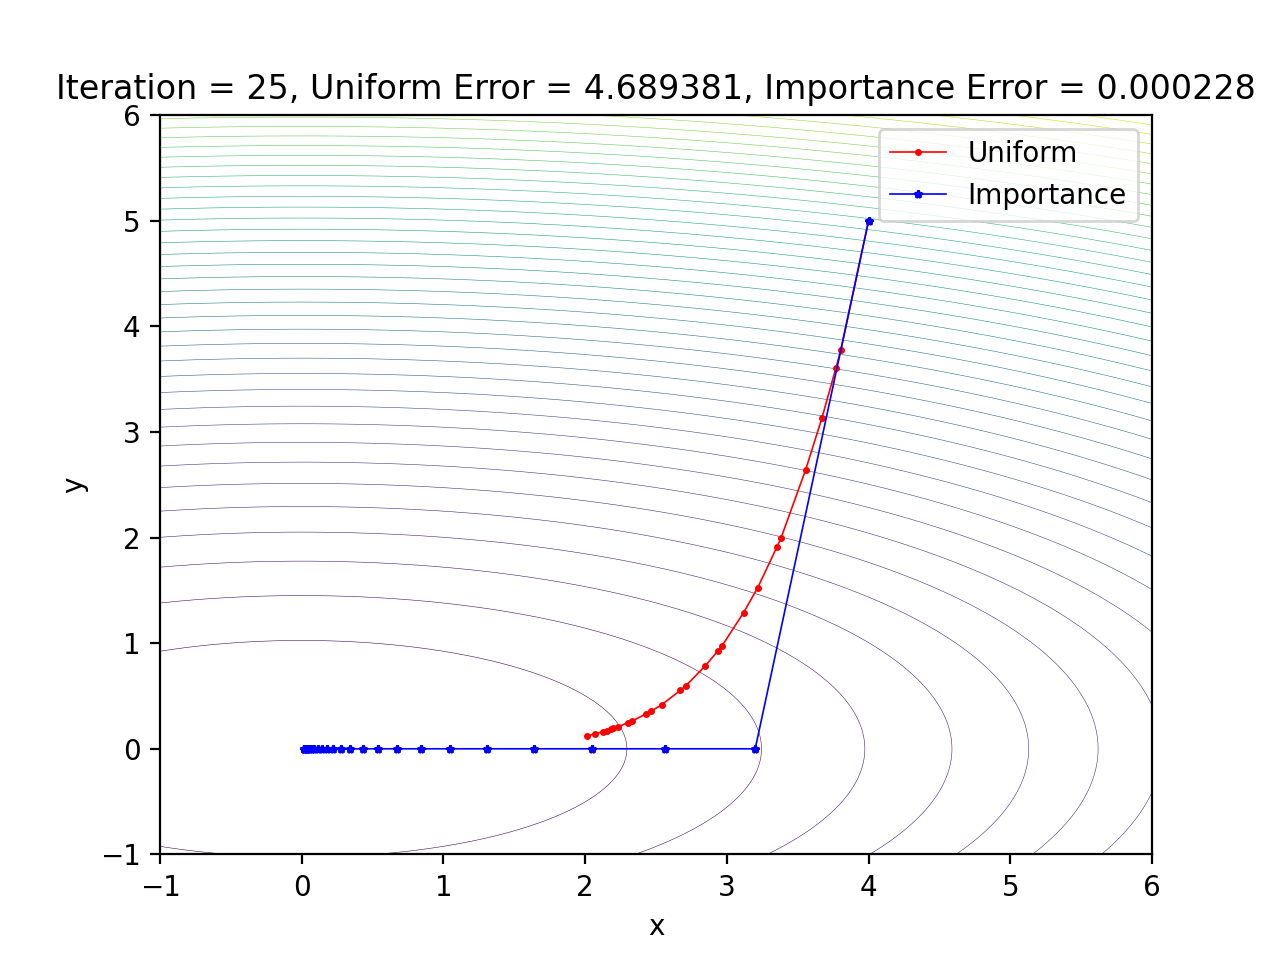
\includegraphics[width=6.7cm]{Figure_34.png}}
	\subfigure[]{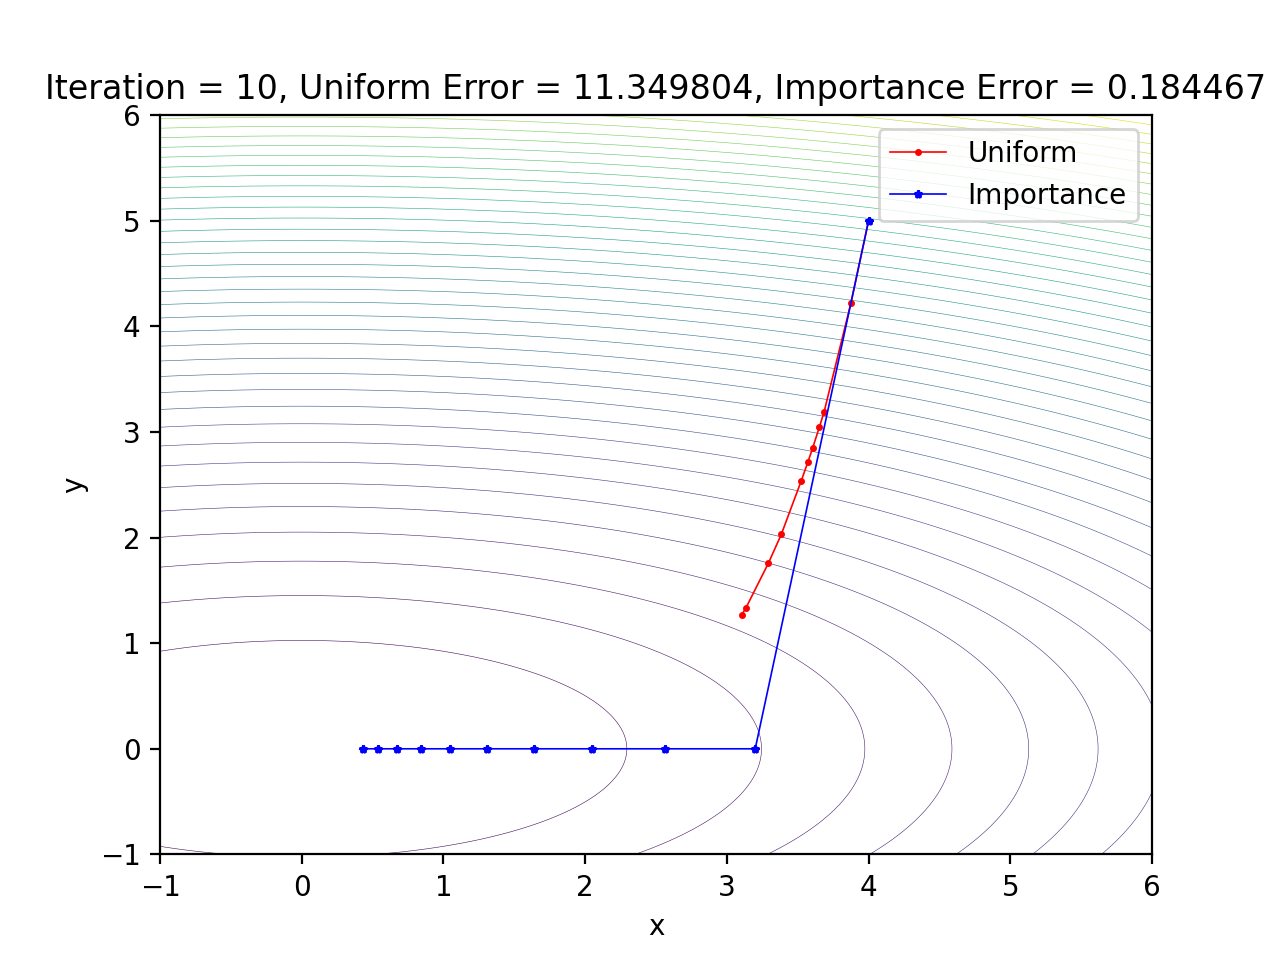
\includegraphics[width=6.7cm]{Figure_35.png}}

	
	\caption{ The trajectories and empirical error of SGD-US and SGD-IS with different iterations, you can see the blue lines converge much faster than the red line.} %图片标题
	\label{img1}
\end{figure}

\paragraph{p3.}
Denote $|S|$ as the cardinality of $S$,  $P_k = C_n^kP(S=U),$ where $U$ is any set whose cardinality is $k$.
We define the unbiased estimator as
\begin{equation}
	g(x) \stackrel{\text { def }}{=} \frac{1}{nP_{|S|}|S|} \sum_{i \in S} \nabla f_{i}(x).
\end{equation}
\begin{theorem}
	The gradient estimator $g$ defined in (2) is unbiased. If we further assume that $n\geq 2,$ $f_i$ is
	convex and $L_i-$smooth for all $i$, and $f$ is $L-$smooth, then 
	\begin{equation}
		\mathrm{E}\left[\|g(x)-g(y)\|^{2}\right] \leq 2 A^{\prime \prime} D_{f}(x, y)
	\end{equation}
where 
\begin{equation}
	A'' =\sum_{k=1}^n \frac{1}{n^2P_k}\left(\frac{n-k}{k(n-1)} \max _{i} L_{i}+\frac{n(k-1)}{k(n-1)} L\right).
\end{equation}
\end{theorem}

\begin{proof}
	\textbf{Unbiasedness.}  Let $\chi_{i}$ be the random variable defined by
	$$
	\chi_{i}= \begin{cases}1 & i \in S \\ 0 & i \notin S\end{cases}
	$$
	It is easy to show that
	$$
	\mathrm{E}\left[\chi_{i}\mid |S|\right]=\frac{|S|}{n}
	$$
	Unbiasedness of $g(x)$ now follows via direct computation:
	$$
	\begin{aligned}
		\mathrm{E}[g(x)] & \stackrel{}{=}\mathrm{E}\left[ \mathrm{E}\left[\frac{1}{nP_{|S|}|S|} \sum_{i \in S} \nabla f_{i}(x)\mid |S|\right]\right]\\
		&=\mathrm{E}\left[\mathrm{E}\left[\frac{1}{nP_{|S|}|S|} \sum_{i=1}^{n} \chi_{i} \nabla f_{i}(x)\mid |S|\right] \right]\\
		&=\mathrm{E}\left[\frac{1}{nP_{|S|}|S|}\sum_{i=1}^{n}\mathrm{E}\left[\chi_{i}\mid |S|\right]\nabla f_i(x)\right]\\
		&=\mathrm{E}\left[\frac{|S|}{n}\frac{1}{nP_{|S|}|S|}\sum_{i=1}^{n}\nabla f_i(x)\right]\\
		&=\frac{1}{n}\sum_{k=1}^{n}P_{k}\left(\frac{1}{nP_{k}}\sum_{i=1}^{n}\nabla f_i(x)\right)\\
		&=\frac{1}{n}\sum_{i=1}^{n}\nabla f_{i}(x)=\nabla f(x).
	\end{aligned}
	$$
	\textbf{Expected smoothness (i.e., computing constant $A^{\prime \prime}$ ).} Fix $x, y \in \mathbb{R}^{d}$ and let
	$$
	a_{i} \stackrel{\text { def }}{=} \nabla f_{i}(x)-\nabla f_{i}(y)
	$$
	Let $\chi_{i j}$ be the random variable defined by
	$$
	\chi_{i j}= \begin{cases}1 & i \in S \text { and } j \in S \\ 0 & \text { otherwise }\end{cases}
	$$
	Note that
	$$
	\chi_{i j}=\chi_{i} \chi_{j}
	$$
	Further, it is easy to show that
	$$
	\mathrm{E}\left[\chi_{i j}\mid |S|\right]=\frac{|S|(|S|-1)}{n(n-1)}
	$$
	It is easy to check that for any vectors $b_{1}, \ldots, b_{n} \in \mathbb{R}^{d}$ we have the identity
	$$
	\left\|\sum_{i=1}^{n} b_{i}\right\|^{2}-\sum_{i=1}^{n}\left\|b_{i}\right\|^{2}=\sum_{i \neq j}\left\langle b_{i}, b_{j}\right\rangle.
	$$
	
	We will use this identity twice in what follows:
	\begin{equation}
	\begin{array}{ll}
		\mathrm{E}\left[\|g(x)-g(y)\|^{2}\right] & \stackrel{}{=} \mathrm{E}\left[\mathrm{E}\left[\left\|\frac{1}{nP_{|S|}|S|} \sum_{i \in S} \nabla f_{i}(x)-\frac{1}{nP_{|S|}|S|} \sum_{i \in S} \nabla f_{i}(y)\right\|^{2}\mid |S|\right]\right] \\
		& \stackrel{}{=}  \mathrm{E}\left[\mathrm{E}\left[\left\|\frac{1}{nP_{|S|}|S|}\sum_{i =1}^{n} \chi_{i}a_{i}\right\|^{2}\mid |S|\right]\right] \\
		& \stackrel{}{=} \mathrm{E}\left[ \mathrm{E}\left[(\frac{1}{nP_{|S|}|S|})^2\sum_{i=1}^{n}\left\|\chi_{i} a_{i}\right\|^{2}+(\frac{1}{nP_{|S|}|S|})^2\sum_{i \neq j}\left\langle\chi_{i} a_{i}, \chi_{j} a_{j}\right\rangle\mid |S|\right] \right]\\
		& \stackrel{}{=} \mathrm{E}\left[\mathrm{E}\left[(\frac{1}{nP_{|S|}|S|})^2\sum_{i=1}^{n}\left\|\chi_{i} a_{i}\right\|^{2}+(\frac{1}{nP_{|S|}|S|})^2\sum_{i \neq j} \chi_{i j}\left\langle a_{i}, a_{j}\right\rangle\mid |S|\right] \right]\\
		& = \mathrm{E}\left[(\frac{1}{nP_{|S|}|S|})^2\left( \sum_{i=1}^{n} E\left[\chi_{i}\mid |S|\right]\left\|a_{i}\right\|^{2}+\sum_{i \neq j} E\left[\chi_{i j}\mid |S|\right]\left\langle a_{i}, a_{j}\right\rangle\right)\right]\\
		&= \mathrm{E}\left[(\frac{1}{nP_{|S|}|S|})^2\left(\sum_{i =1}^n\frac{|S|}{n}\left\|a_i\right\|^2+\sum_{i \neq j}\frac{|S|(|S|-1)}{n(n-1)}\langle a_i,a_j\rangle \right)\right]\\
		&=\mathrm{E}\left[(\frac{1}{nP_{|S|}})^2\left(\frac{1}{|S|n}\sum_{i =1}||a_i||^2+\frac{|S|-1}{|S|n(n-1)}\sum_{i \neq j}\langle a_i,a_j\rangle \right)\right]\\
		&=\mathrm{E}\left[(\frac{1}{nP_{|S|}})^2\left(\frac{1}{|S| n} \sum_{i=1}^{n}\left\|a_{i}\right\|^{2}+\frac{|S|-1}{|S| n(n-1)}\left(\left\|\sum_{i=1}^{n} a_{i}\right\|^{2}-\sum_{i=1}^{n}\left\|a_{i}\right\|^{2}\right)\right)\right]\\
		&=\mathrm{E}\left[(\frac{1}{nP_{|S|}})^2\left(\frac{n-|S|}{|S|(n-1)} \frac{1}{n} \sum_{i=1}^{n}\left\|a_{i}\right\|^{2}+\frac{n(|S|-1)}{|S|(n-1)}\left\|\frac{1}{n} \sum_{i=1}^{n} a_{i}\right\|^{2}\right)\right]
	\end{array}
	\end{equation}
	Since $f_{i}$ is convex and $L_{i}$-smooth, we know that
	$$
	\left\|a_{i}\right\|^{2} \stackrel{}{=}\left\|\nabla f_{i}(x)-\nabla f_{i}(y)\right\|^{2} \leq 2 L_{i} D_{f_{i}}(x, y)
	$$
	Since $f$ is convex and $L$-smooth, we know that
	$$
	\left\|\frac{1}{n} \sum_{i=1}^{n} a_{i}\right\|^{2} \stackrel{}{=}\|\nabla f(x)-\nabla f(y)\|^{2} \leq 2 L D_{f}(x, y)
	$$
	It only remains to plug these bounds to $(5)$, apply the bound $L_{i} \leq \max _{i} L_{i}$ and use the identity $D_{f}(x, y)=\frac{1}{n} \sum_{i=1}^{n} D_{f_{i}}(x, y):$
	$$
	\begin{aligned}
		\mathrm{E}\left[\|g(x)-g(y)\|^{2}\right] & \stackrel{}{\leq} \mathrm{E}\left[(\frac{1}{nP_{|S|}})^2\left(\frac{n-|S|}{|S|(n-1)} \frac{1}{n} \sum_{i=1}^{n} 2 L_{i} D_{f_{i}}(x, y)+\frac{n(|S|-1)}{|S|(n-1)} 2 L D_{f}(x, y)\right)\right] \\
		& \leq 2\mathrm{E}\left[(\frac{1}{nP_{|S|}})^2\left( \frac{n-|S|}{|S|(n-1)} \max _{i} L_{i} \frac{1}{n} \sum_{i=1}^{n} D_{f_{i}}(x, y)+2 \frac{n(|S|-1)}{|S|(n-1)} L D_{f}(x, y) \right)\right]\\
		&=2\mathrm{E}\left[(\frac{1}{nP_{|S|}})^2\left( \frac{n-|S|}{|S|(n-1)} \max _{i} L_{i} D_{f}(x, y)+2 \frac{n(|S|-1)}{|S|(n-1)} L D_{f}(x, y)\right)\right] \\
		&=2\mathrm{E}\left[(\frac{1}{nP_{|S|}})^2\left(\frac{n-|S|}{|S|(n-1)} \max _{i} L_{i}+\frac{n(|S|-1)}{|S|(n-1)} L\right) D_{f}(x, y)\right]\\
		&=\left(2\sum_{k=1}^n P_k(\frac{1}{nP_k})^2\left(\frac{n-k}{k(n-1)} \max _{i} L_{i}+\frac{n(k-1)}{k(n-1)} L\right) \right)D_{f}(x, y) \\
		&=\left(2\sum_{k=1}^n \frac{1}{n^2P_k}\left(\frac{n-k}{k(n-1)} \max _{i} L_{i}+\frac{n(k-1)}{k(n-1)} L\right)\right) D_{f}(x, y),
	\end{aligned}
	$$
	so $A'' =\sum_{k=1}^n \frac{1}{n^2P_k}\left(\frac{n-k}{k(n-1)} \max _{i} L_{i}+\frac{n(k-1)}{k(n-1)} L\right)$.
	
\end{proof}

\paragraph{p4.}
In my experiments(see Figure\ref{img2}.), I set $d = 1, n = 10, \epsilon = 10^{-4},  f(x)=\frac{1}{ 10} \sum_{i=1}^{10} f_i(x), f_i(x) = \frac{1}{2}\left\|a_{i}^{} x-b_{i}\right\|_{2}^{2}$, $a = [2,4,6,3,2,9,6,7,11,45], b = [1,2,3,4,5,6,7,8,9,11]$, based on these information, we can get that $x_{\star} = 0.3343133137337253, \sigma_{\star}^2 = 3993.739347850591, \max_{i} L_i = 2025, L = \mu = 238.1, $ then insert this information into the following formula 
\begin{equation*}
	\tau^{\star}=\frac{n\left(\theta+L-\max _{i} L_{i}\right)}{\theta+n L-\max _{i} L_{i}}, \text{ where } \theta=\frac{2 \sigma_{\star}^{2}}{\varepsilon \mu},
\end{equation*}
we get $\tau_{\star} = 9.936$, then we calculate the value of 
$$\mathcal{C}(\tau) \stackrel{}{=} \frac{2}{\mu(n-1)} \max \{(n-\tau) \max _{i} L_{i}+n(\tau-1) L, (n-\tau) \frac{2 \sigma_{\star}^{2}}{\varepsilon \mu}\}, \text{  for }\tau = 9,10,$$
we get $\mathcal{C}(9)= 335467.3958715322>\mathcal{C}(10) = 21429$, so $\tau_{\star} = 10.$ I sample 100 points in the last step to estimate $\mathrm{E}\left[||x_{\text{last step}}-x_{\star}||^2\right]$
\begin{figure}
	\centering
	\subfigure[ ]{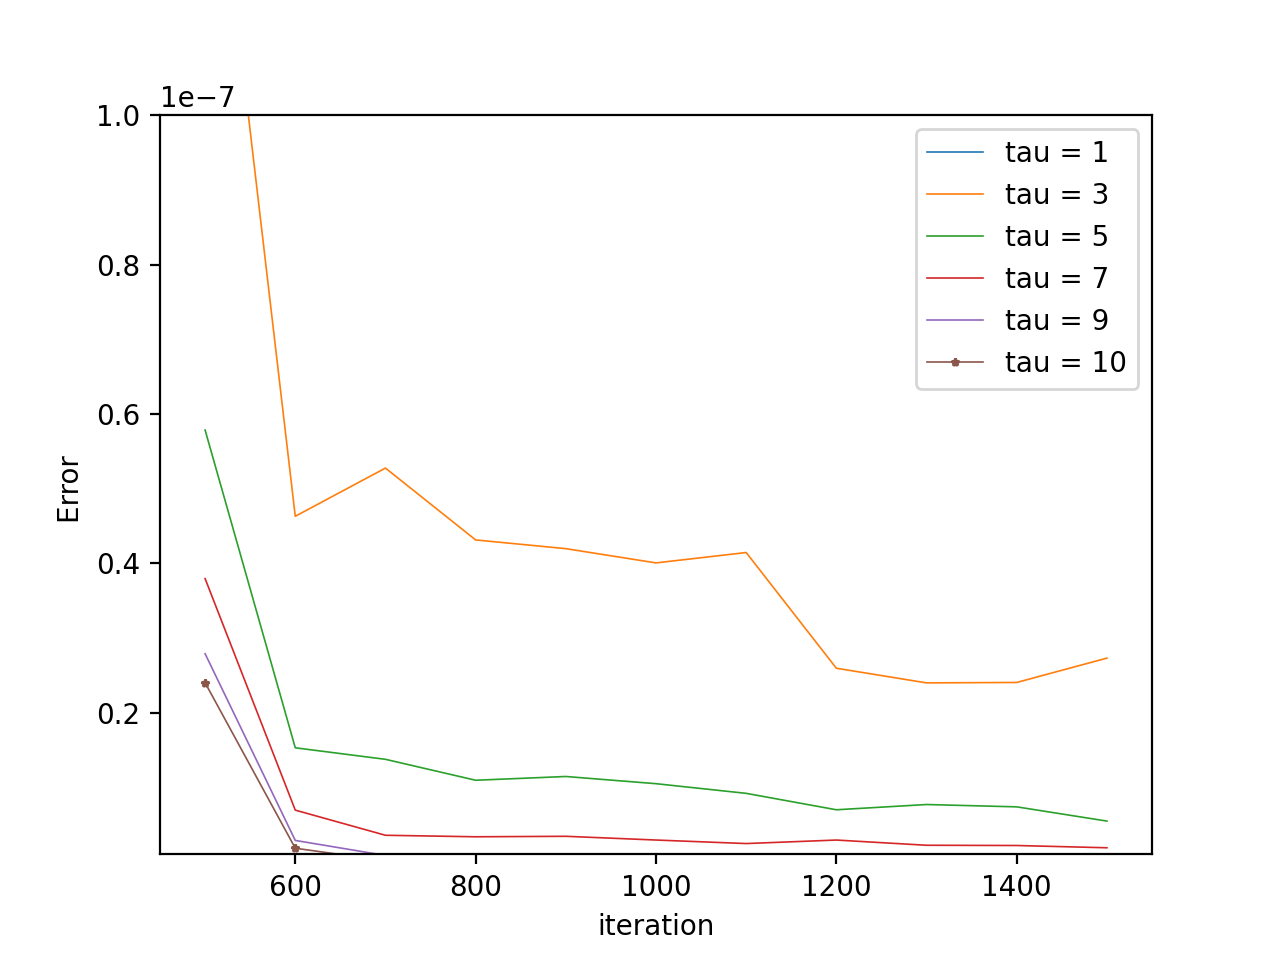
\includegraphics[width=6.7cm]{Figure_347.png}} 
	\subfigure[]{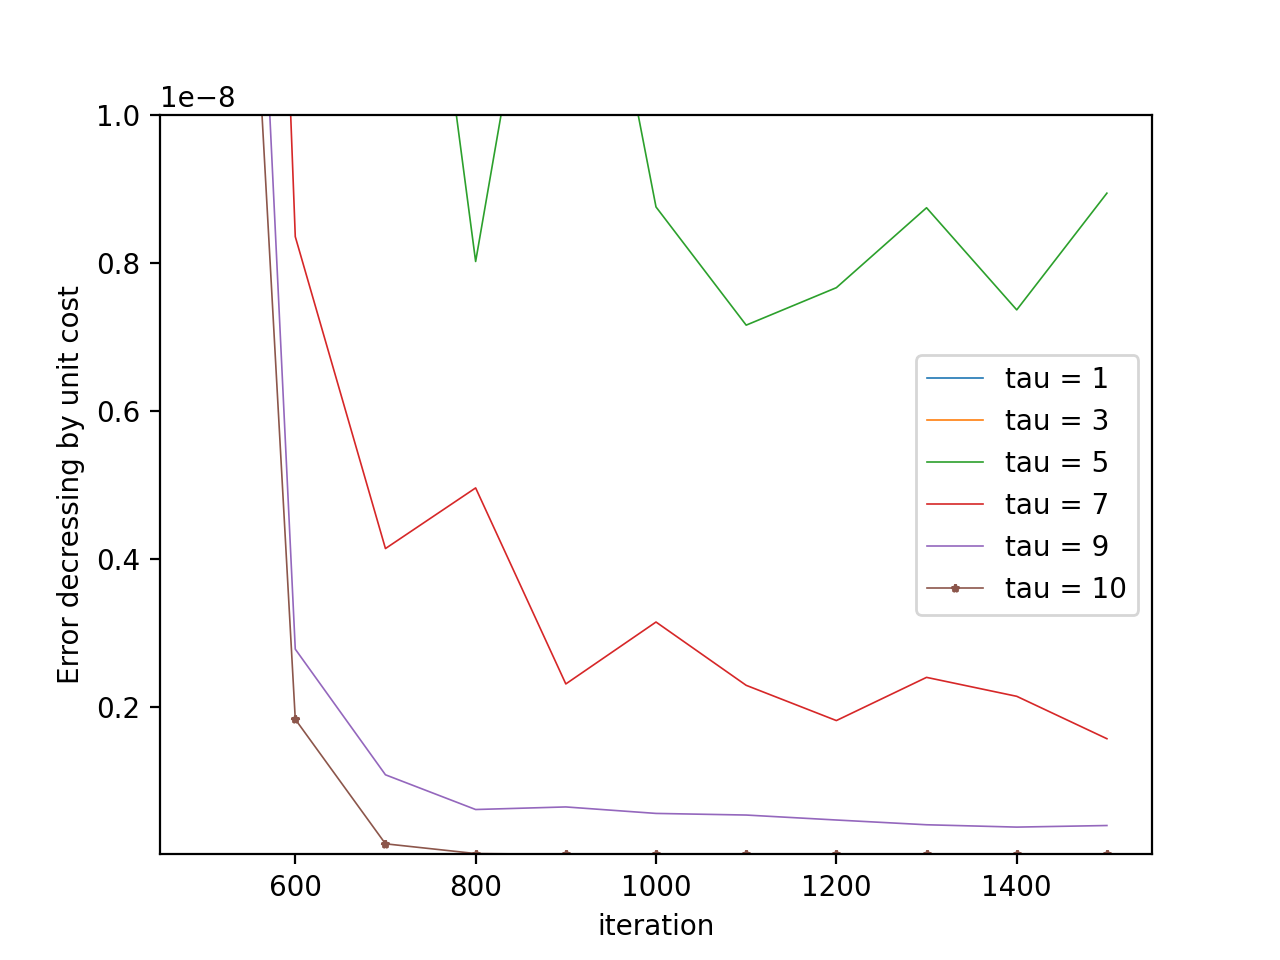
\includegraphics[width=6.7cm]{Figure_356.png}}
	\\ %换行
	
	
	\caption{ Note some line are not in the plot, since their values are bigger than the upper limit of y-axis. In picture (a), the y-axis is the mean square distance from the minimum point sampled from the last step, in picture (b), I divide the error by (step times tau), which means the error decreasing by unit cost, the lower the value, means the better of the choice of tau. In both plots, you can see the line of tau equals 10 achieves the lowest value. } %图片标题
	\label{img2}
\end{figure}


\paragraph{p5.}
\begin{proof}{}
As before, let $\chi_{i}$ be the random variable defined by
	$$
	\chi_{i}= \begin{cases}1 & i \in S \\ 0 & i \notin S\end{cases}
	$$
	It is easy to show that
	$$
	\mathrm{E}\left[\chi_{i}\right]=\operatorname{Prob}(i \in S)=\operatorname{Prob}\left(i \in S_{i}\right)=p_{i}
	$$

	$$
	\mathrm{E}\left[\chi_{i}\chi_j\right]=\mathrm{E}\left[\chi_i\right]\mathrm{E}\left[\chi_j\right]=p_{i}p_{j}, \text{   for } i\neq j,
	$$


denote $a_i(x)=\nabla f_i(x)$, $\mathrm{E}\left[||g(x)||^2\right]$ now follows via direct computation:
	$$
	\begin{aligned}
		\mathrm{E}[||g(x)||^2] & \stackrel{}{=} \mathrm{E}\left[||\sum_{i \in S} \frac{1}{n p_{i}} \nabla f_{i}(x)||^2\right] \\
		&=\frac{1}{n^2}\mathrm{E}\left[||\sum_{i=1}^{n} \chi_{i} \frac{1}{p_i}a_i(x)||^2\right] \\
		&=\frac{1}{n^2}\mathrm{E}\left[\sum_{i =1}^{n}\frac{1}{p_i^2}||\chi_ia_i(x)||^2+\sum_{i\neq j}\frac{1}{p_ip_j}\langle \chi_ia_i(x),\chi_ja_j(x)\rangle\right] \\
		& \stackrel{}{=} \frac{1}{n^2}\left(\sum_{i =1}^{n}\frac{1}{p_i^2}||a_i(x)||^2\mathrm{E}\left[\chi_i\right]+\sum_{i \neq j}\frac{1}{p_ip_j}\mathrm{E}\left[\chi_i\chi_j\right]\langle a_i(x),a_j(x)\rangle \right)\\
		&=\frac{1}{n^2}\left(\sum_{i =1}^n\frac{1}{p_i}||a_i(x)||^2+\sum_{i \neq j}\langle a_i(x),a_j(x)\rangle\right)\\
		&=\frac{1}{n^2}\left(\sum_{i =1}^n\frac{1}{p_i}||a_i(x)||^2+||\sum_{i =1}^na_i(x)||^2-\sum_{i =1}^n||a_i(x)||^2\right)\\
		&=\frac{1}{n^2}\left(\sum_{i =1}^n\left(\frac{1}{p_i}-1\right)||a_i(x)||^2+||\sum_{i =1}^na_i(x)||^2\right)\\
		&=\frac{1}{n^2}\left(\sum_{i =1}^n\left(\frac{1}{p_i}-1\right)||\nabla f_i(x)||^2+||\sum_{i =1}^n\nabla f_i(x)||^2\right)\\
		&=||\nabla f(x)||^2+\frac{1}{n^2}\sum_{i =1}^n\left(\frac{1}{p_i}-1\right)||\nabla f_i(x)||^2
	\end{aligned}
	$$
\end{proof}


\end{document}